\documentclass[ngerman,aspectratio=169]{beamer}
\usepackage[utf8]{luainputenc}
\usepackage[TS1,T1]{fontenc}
\usepackage{babel}
\usetheme[pagenum,navbar,ddc]{tud}
\usepackage{xcolor}
\usepackage{listings}
\usepackage{tikz}
\usepackage{multicol}
\usepackage[labelformat=empty,font=scriptsize]{caption}
\usepackage{marvosym}

\newcommand{\theory}[1]{\text{Th(} #1 \text{)}}
\newcommand{\lang}[1]{\text{L(}#1{)}}

\title{TUN/TAP-Geräte \protect\\\mdseries Übersicht, Funktionsweise und Implementierung im Linux-Kernel\strut}
\subtitle{Proseminar Rechnernetze}
\author{Lucas Waclawczyk}

\newcommand*\inmm[1]{\pgfmathsetmacro\inmmwert{#1 / 1mm}\inmmwert}
\makeatletter
\newcommand*\inpt[1]{\setlength\@tempdima{#1}\the\@tempdima}
\makeatother

\AtBeginSection[]{\partpage{\usebeamertemplate***{part page}}}
\begin{document}
	\mode<presentation>{\setbeamertemplate{tud background}[image/shaded]{Seminarraum.jpg}{0.7}}
	\maketitle
	
	\mode<presentation>{\setbeamertemplate{page number in footline}[frame][text and total]}
	\frame{\frametitle{Inhalt}\tableofcontents}
	
	\section{Übersicht}
	\subsection{Rückblick Network Interfaces}
	\begin{frame}{Rückblick Network Interfaces}
		\only<1-3,5->{
			\begin{multicols}{2}
				\begin{itemize}
					\setlength{\itemsep}{1em}
					\item Interface = Schnittstelle
					\item zwischen zwei Schichten im OSI-Modell
					\visible<3,5->{
						\item übernimmt Daten von Instanz eines {$ (n+1) $-Protokolls}
						\item stellt Daten für Instanz eines {$ (n) $-Protokolls} bereit
					}
					\visible<5->{
						\item muss nicht physisch sein\\
						\MVRightArrow \: Virtual Network Interface
					}
				\end{itemize}
					\only<1>{\hspace{-.5cm}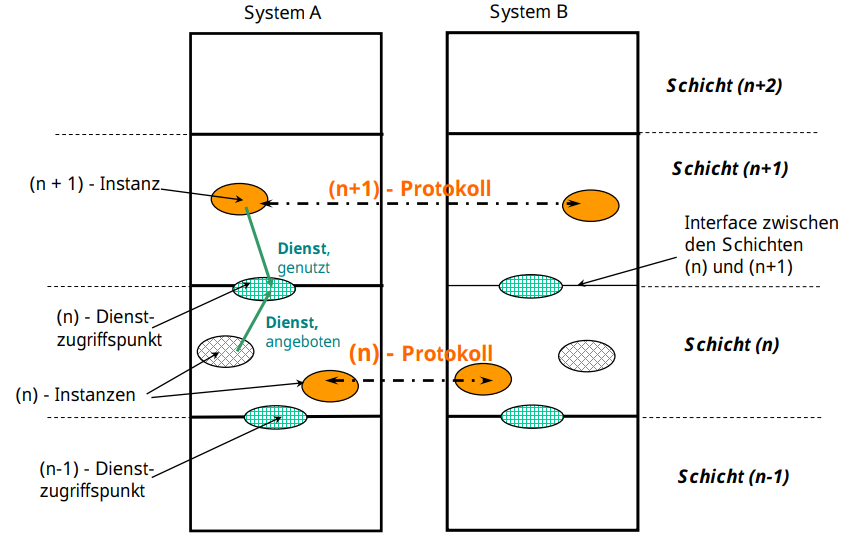
\includegraphics[width=1.2\linewidth]{network_interface}}
					\only<2,3,5->{\hspace{-.5cm}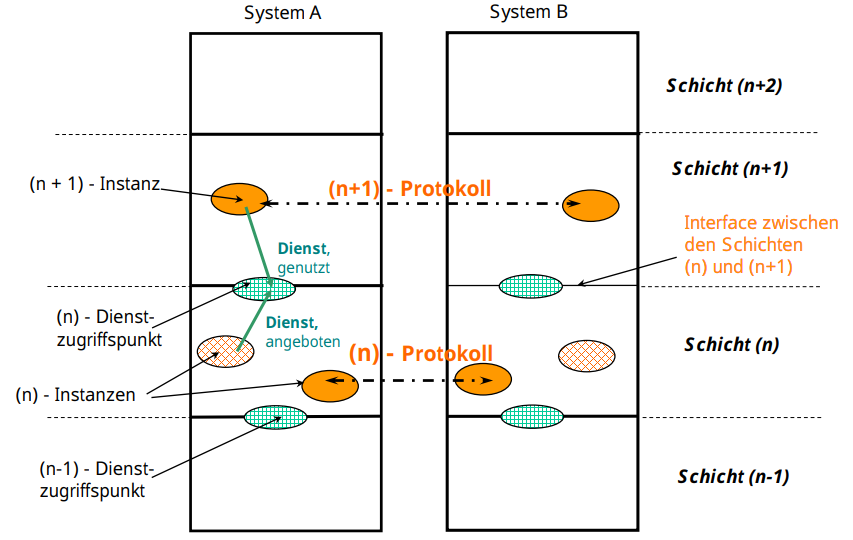
\includegraphics[width=1.2\linewidth]{network_interface_colored}}
					\centering aus \hyperlink{ref:rene}{[1]}
			\end{multicols}
		}
		\only<4>{
			\centering 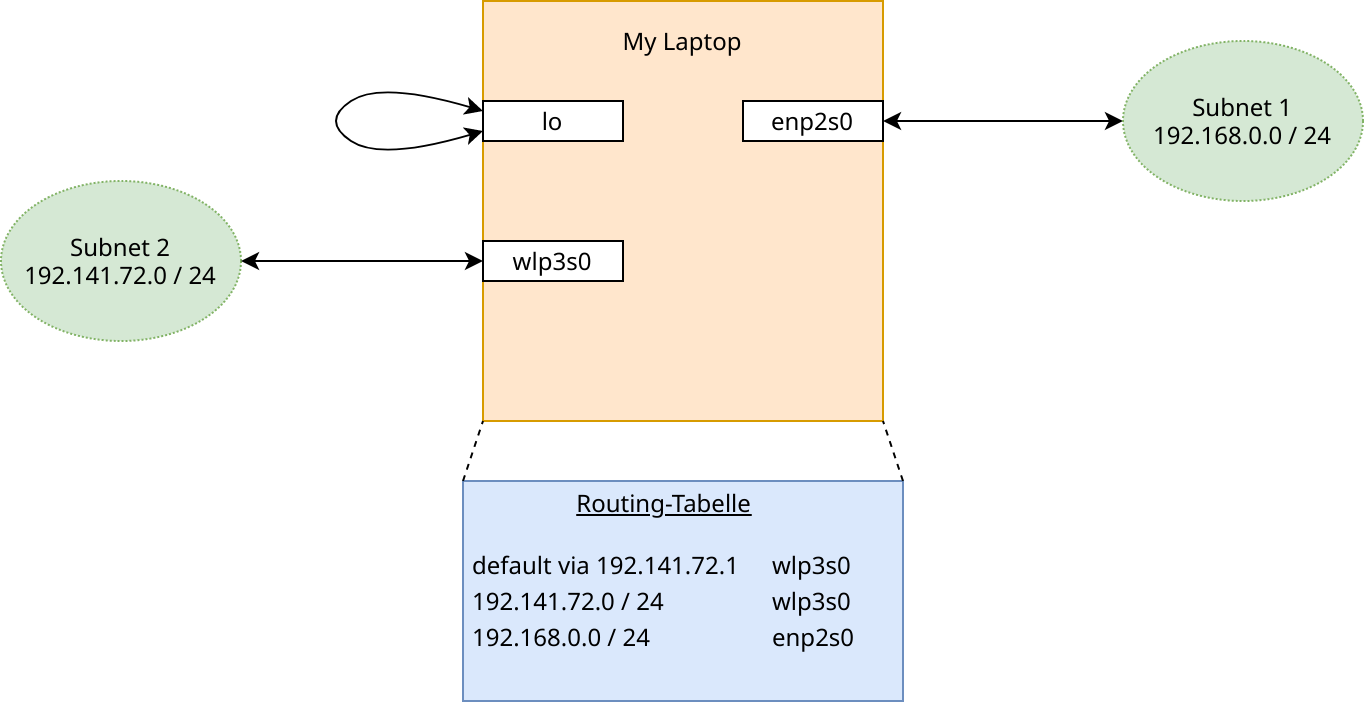
\includegraphics[width=.8\textwidth]{interfaces01}%
		}
	\end{frame}

	\subsection{Generelles zu TUN und TAP}
	\begin{frame}{Generelles zu TUN und TAP}
		\only<1,2,4->{
			\begin{itemize}
				\item Virtual Network Interfaces, d.h. man kann
				\begin{itemize}
					\item[\dots] ihnen IP-Adressen zuweisen
					\item[\dots] ihren Traffic analysieren
					\item[\dots] Firewall-Regeln für sie konfigurieren
					\item[\dots] uvm.
				\end{itemize}
				\visible<2,4->{
					\item \textit{Interface $ \leftrightarrow $ Anwendung} \:\: statt \:\: \textit{Interface $ \leftrightarrow $ physische Verbindung}
				}
				\visible<4->{
					\item u. A. Linux, Windows 2000 - 10, Mac OS X (nur TUN eingebaut)
					\item hier für Linux
				}
			\end{itemize}
		}
		\only<3>{
			\centering 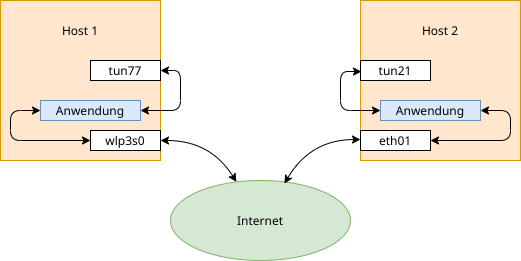
\includegraphics[width=.8\linewidth]{connection}%
		}
	\end{frame}

	\subsection{Vor- und Nachteile}
	\begin{frame}{Vor- und Nachteile \hyperlink{ref:openvpn}{[7]}}
		\only<1-3,6-7>{
			\begin{multicols*}{2}
				\textbf{TAP --  Terminal Access Point}\\
				$ \sim $ Ethernet $ \sim $ Layer 2
				\begin{itemize}
					\visible<2->{
						\item[$ \oplus $] verhält sich wie echter Netzwerkadapter
						\item[$ \oplus $] flexible Protokollwahl
						\item[$ \oplus $] Bridging möglich
					}
					\visible<3->{
						\item[$ \ominus $] viel Overhead (Ethernet-Header, Broadcast)
						\item[$ \ominus $] skaliert schlecht
						\item[$ \ominus $] kein Support bei Android, iOS
					}
				\vspace{3cm}
			
				\textbf{TUN -- Netzwerk-Tunnel}\\
				$ \sim $ IP $ \sim $ Layer 3
				\begin{itemize}
					\visible<6->{
						\item[$ \oplus $] weniger Overhead (kein Ethernet-Header, kein Broadcast)
						\item[$ \oplus $] nur Layer-3-Pakete
					}
					\visible<7->{
						\item[$ \ominus $] nur Layer-3-Pakete
						\item[$ \ominus $] keine Broadcasts
						\item[$ \ominus $] kein Bridging möglich
					}
				\end{itemize}
				\end{itemize}
			\end{multicols*}
		}
	\only<4>{
		\centering 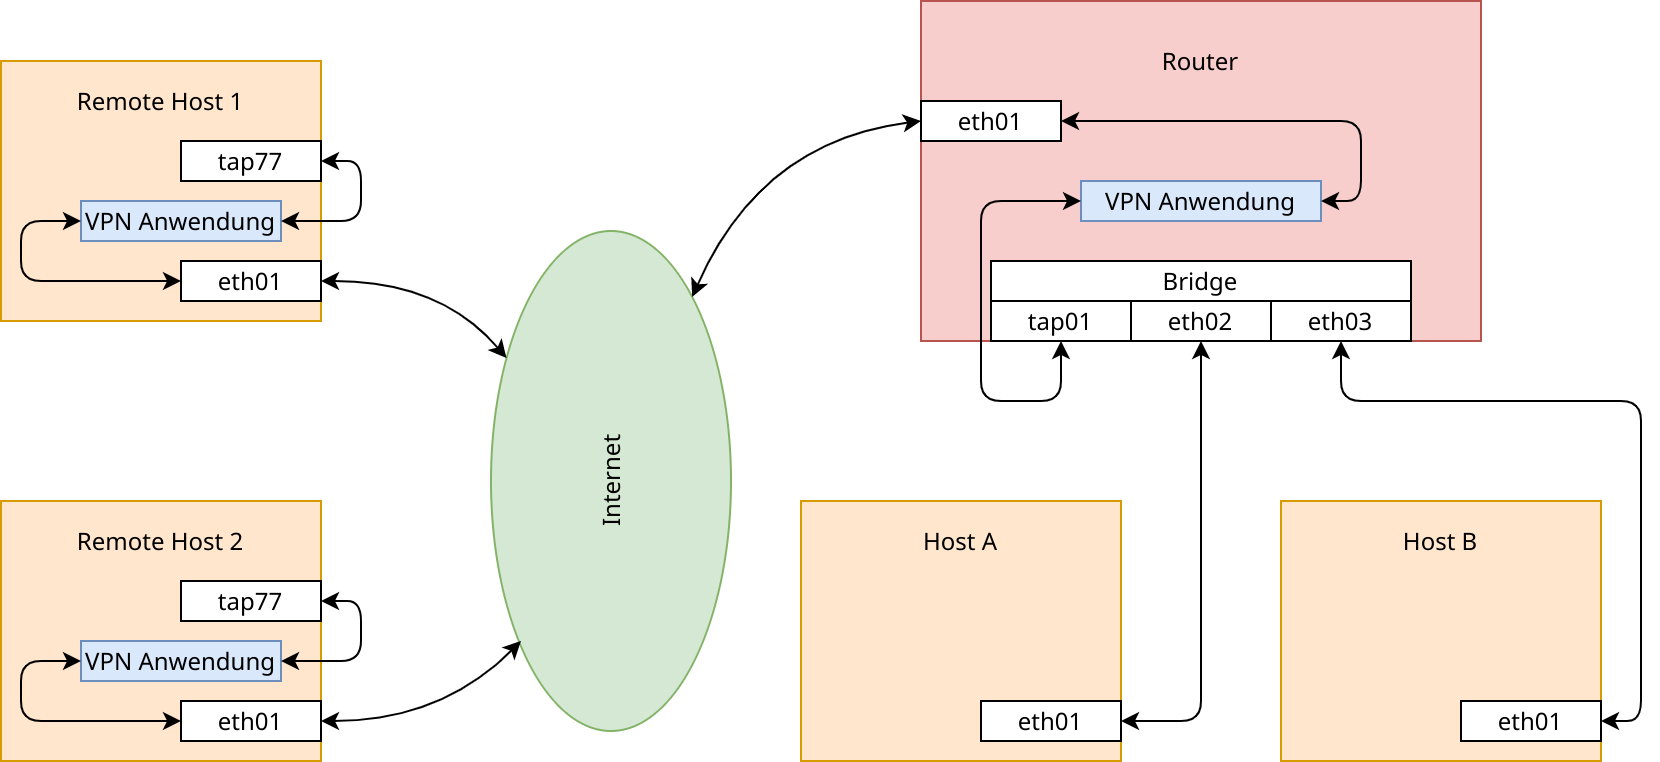
\includegraphics[width=\linewidth]{tap_physical}
	}
	\only<5>{
		\centering 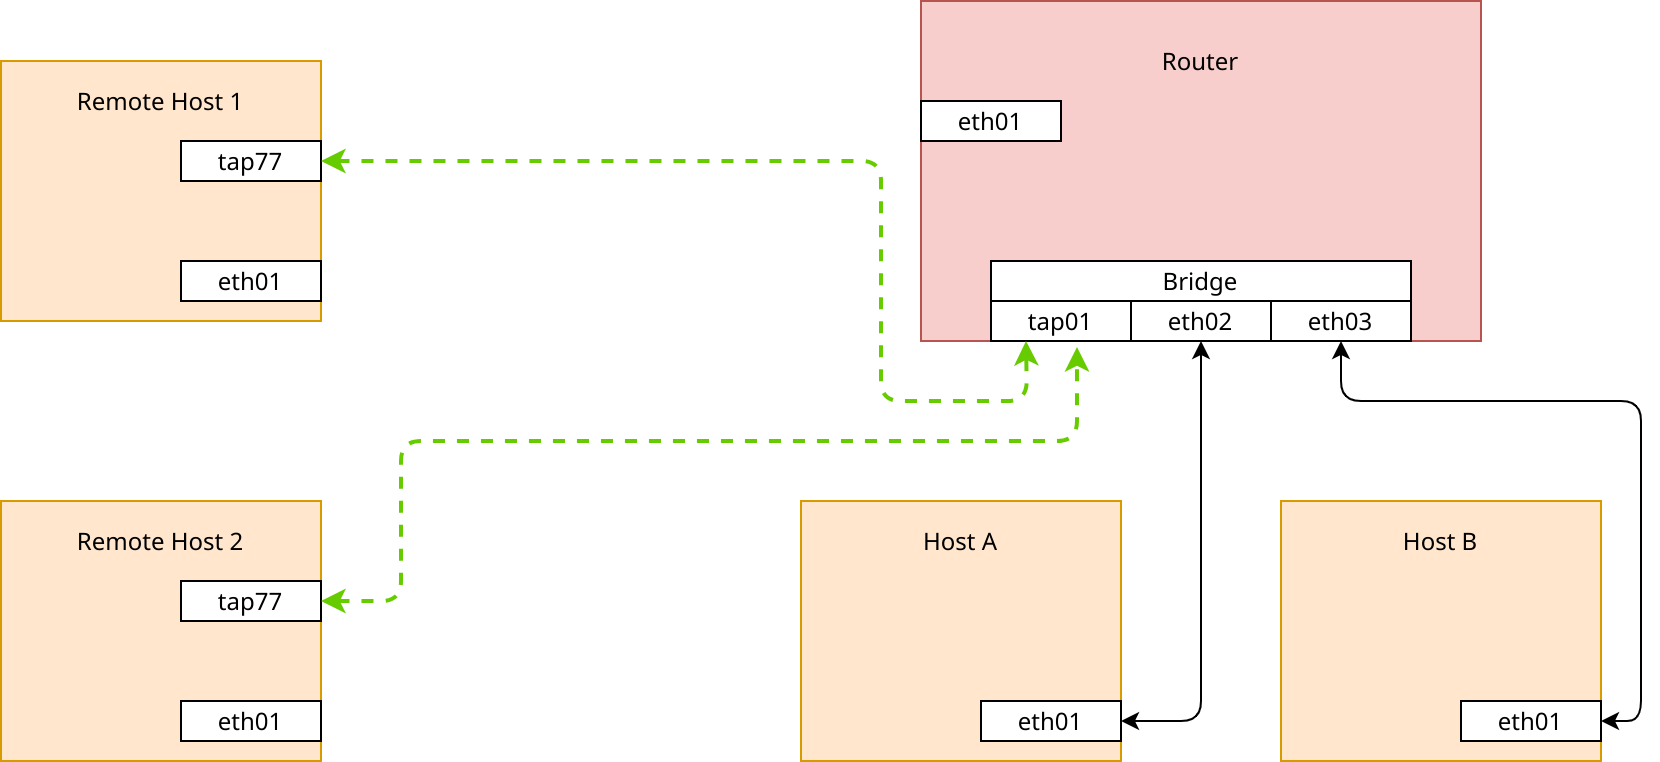
\includegraphics[width=\linewidth]{tap_virtual}
	}
	\only<8>{
		\centering 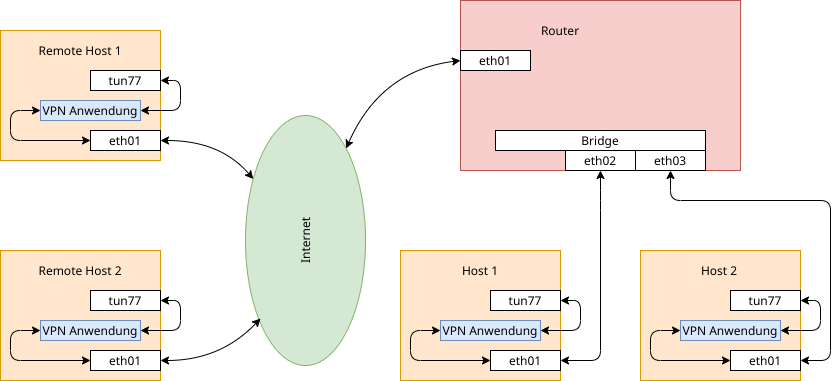
\includegraphics[width=\linewidth]{tun_physical}
	}
	\only<9>{
		\centering 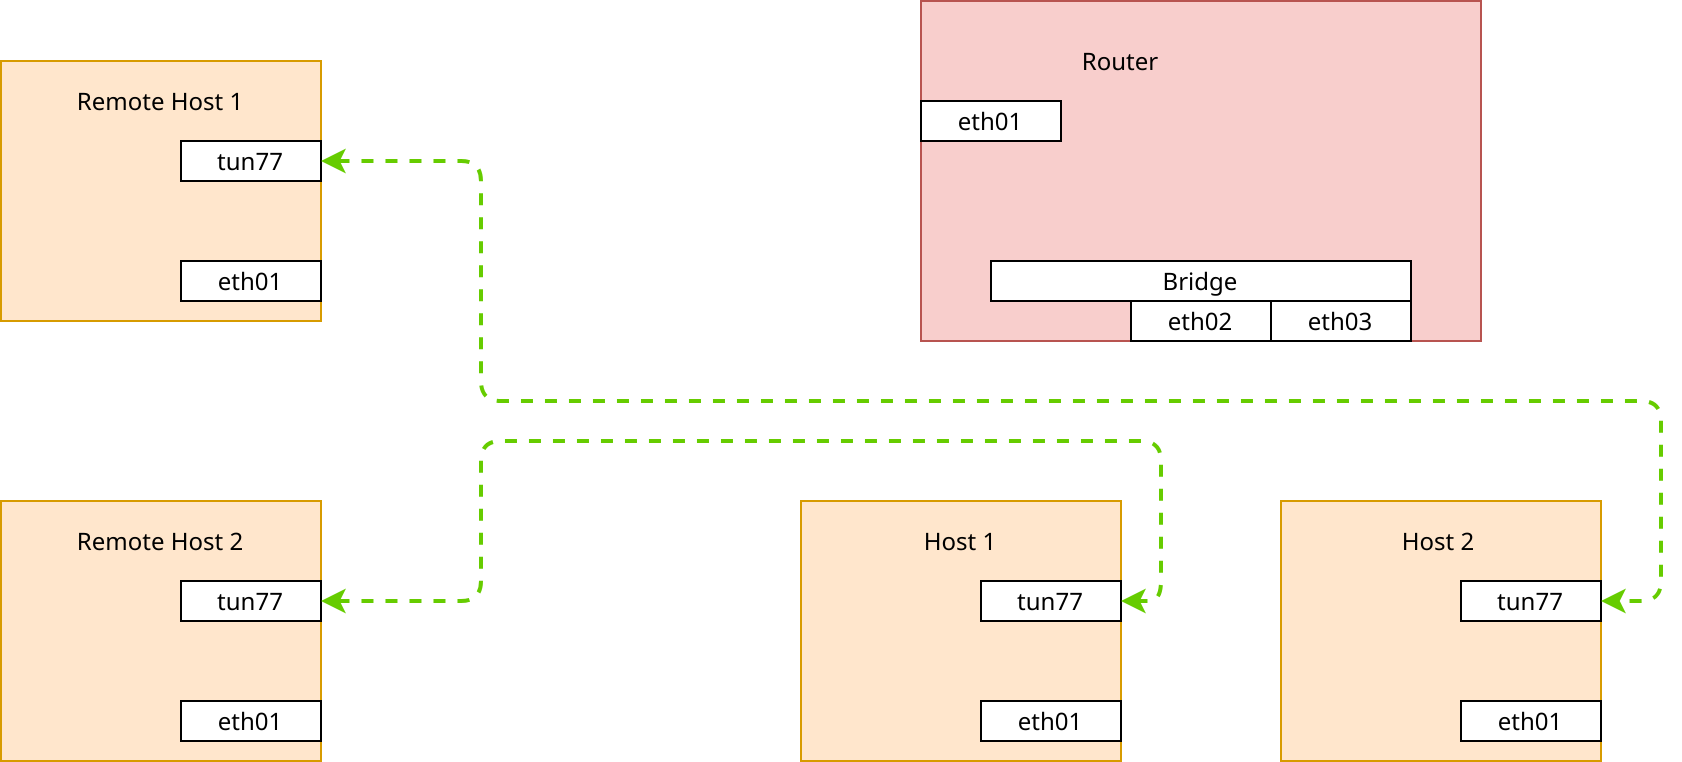
\includegraphics[width=\linewidth]{tun_virtual}
	}
	\end{frame}

	\section{Funktionsweise}
	\subsection{Set Up}
	\begin{frame}{Set Up}
		\only<1,6>{
			Interface erzeugen (erfordert CAP\_NET\_ADMIN capability):
			
			\begin{enumerate}
				\item \texttt{/dev/net/tun} (Clone Device) öffnen (r, w)
				\item Systemaufruf: \texttt{ioctl(fd, TUNSETIFF, options)}
				\item ggf. persistent einrichten
			\end{enumerate}
			\visible<6>{
				\vspace{.3cm}
				VPN Anwendung anbinden:
				
				\begin{itemize}
					\item wiederhole obiges als beliebiger Nutzer
					\item nutze bestehenden Interface-Namen
				\end{itemize}
			}
		}
		\only<2>{\centering 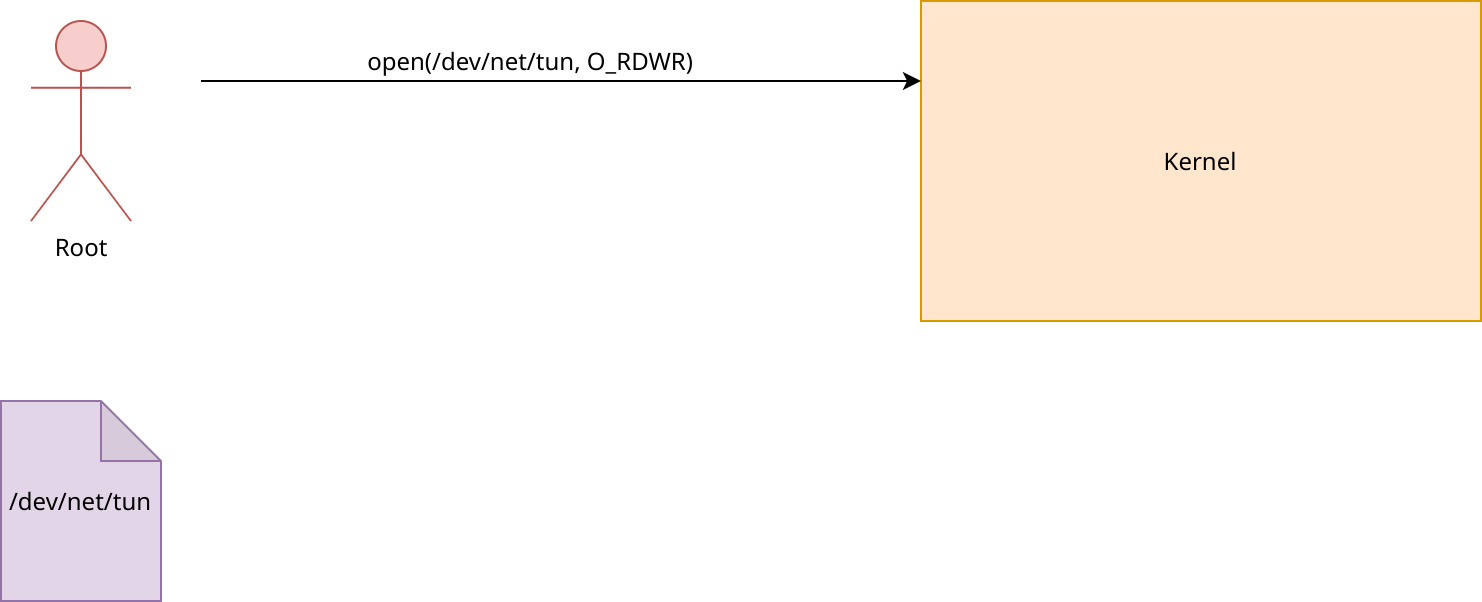
\includegraphics[width=\textwidth]{open_tun01}}
		\only<3>{\centering 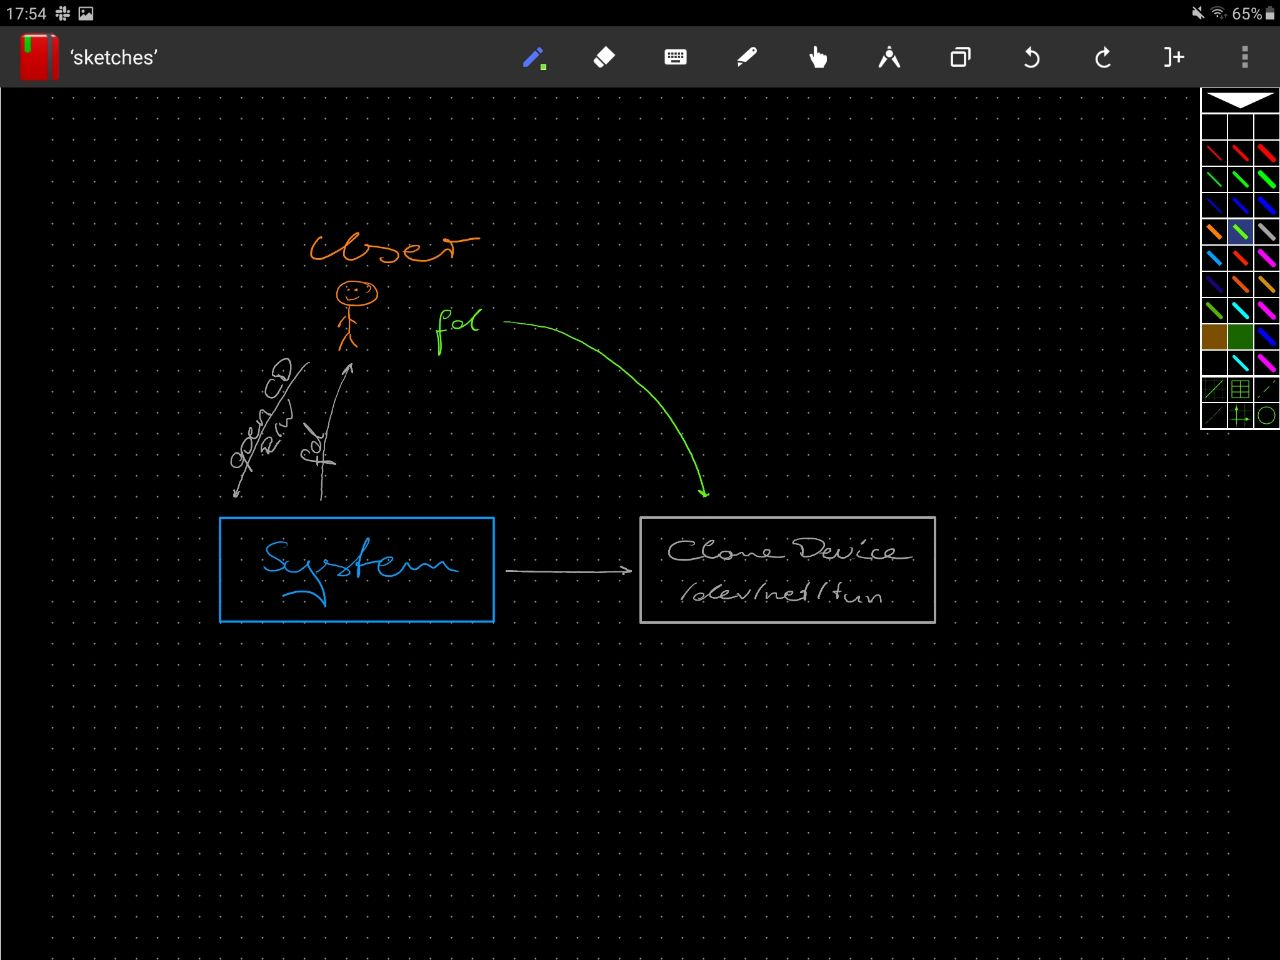
\includegraphics[width=\textwidth]{open_tun02}}
		\only<4>{\centering 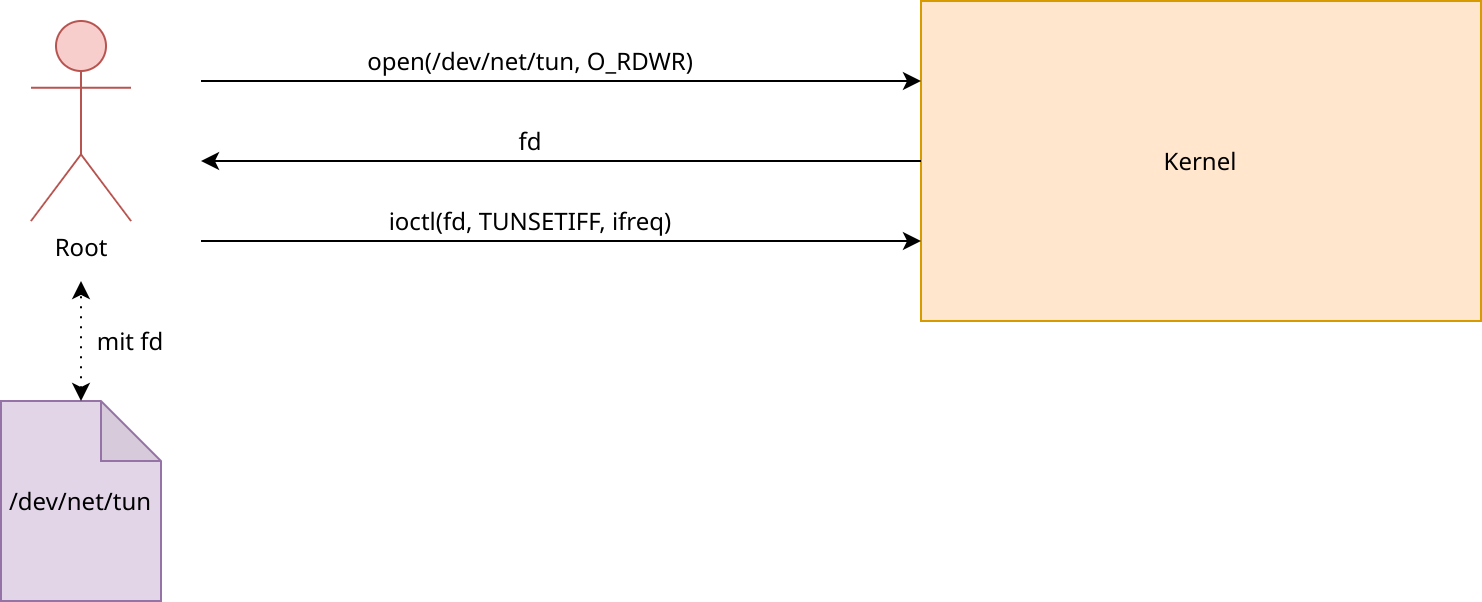
\includegraphics[width=\textwidth]{open_tun03}}
		\only<5>{\centering 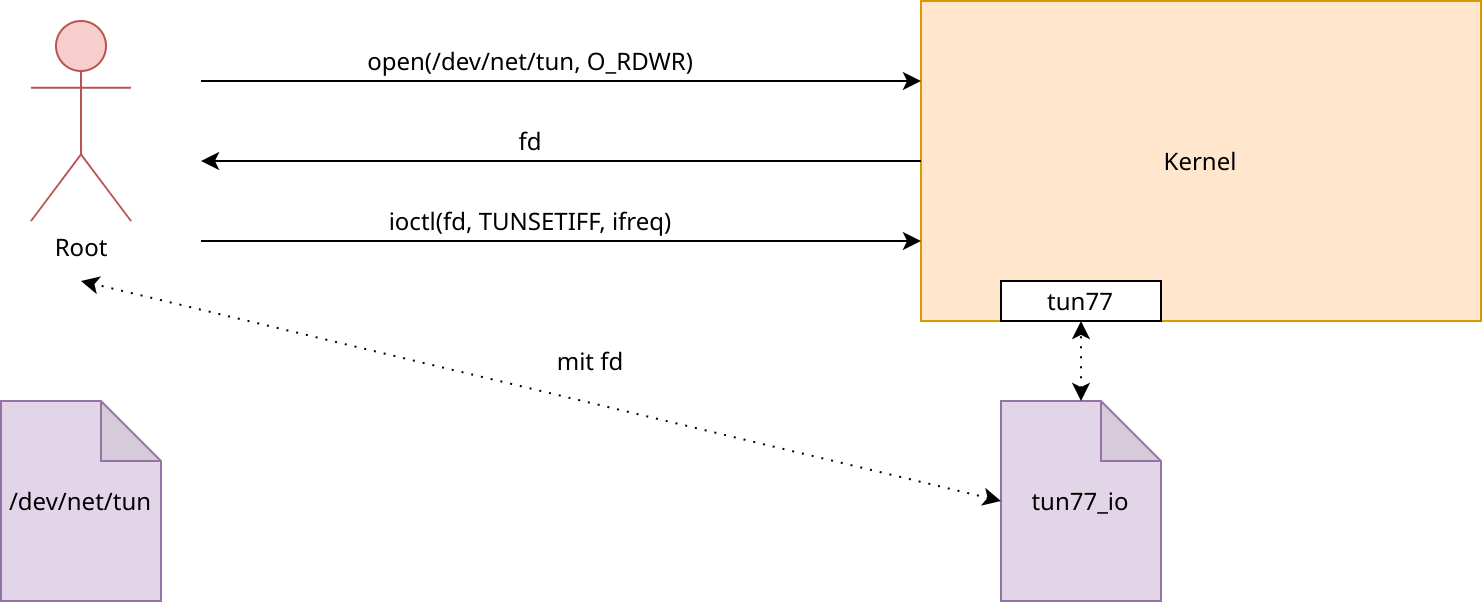
\includegraphics[width=\textwidth]{open_tun04}}
	\end{frame}

	\subsection{Workflow}
	\begin{frame}{Workflow}
		\only<1>{
			\begin{itemize}
				\item 
				
				\item Vorteile
				\begin{itemize}
					\item gut konfigurierbar
					\item verhält sich wie echter Netzwerkadapter
				\end{itemize}
				\item Nachteile
				\begin{itemize}
					\item ineffizient
					\item langsamer als Heimnetz (schwächstes Glied)
				\end{itemize}
			\end{itemize}
		}
		\only<2>{
			\centering 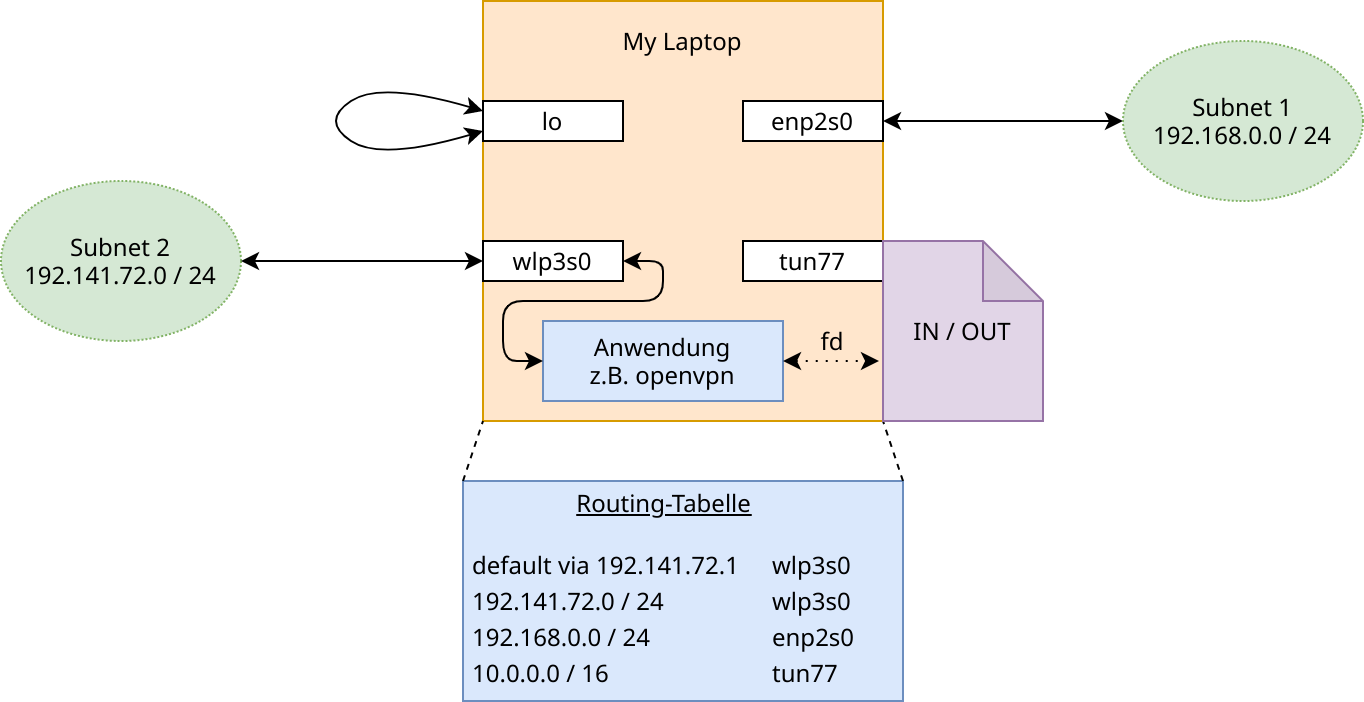
\includegraphics[width=.8\textwidth]{interfaces02}%
		}
	\end{frame}

	\subsection{Tear Down}
	\begin{frame}{Tear Down}
		\begin{itemize}
			\item \emph{transientes} Gerät verschwindet bei Beenden der angebundenen Anwendung
			\item \emph{persistentes} Gerät muss aktiv abgebaut werden
		\end{itemize}
	\end{frame}

	\section{Implementierung}
	\subsection{Wo findet man das?}
	\begin{frame}{Wo findet man das?}
		\begin{itemize}
			\item Kernel-Code: \url{https://github.com/torvalds/linux.git}
			\item TUN: \texttt{/linux/drivers/net/tun.c}
			\item Clone Device: \texttt{/dev/net/tun}
		\end{itemize}
	\end{frame}
	
	\subsection{Code}
	\begin{frame}{Code}
		etwa drei Folien
	\end{frame}

	\section{Quellen}
	\begin{frame}{Quellen}
		\begin{enumerate}
			\item[{[1]}] Skript und Übungsaufgaben der Vorlesung Rechnernetze, TU Dresden 2019 (präzise genug?) \label{ref:rene}
			\item[{[2]}] \url{https://backreference.org/2010/03/26/tuntap-interface-tutorial/}
			\item[{[3]}] \url{https://www.elektronik-kompendium.de/sites/net/0811011.htm}
			\item[{[4]}] \url{https://en.wikipedia.org/wiki/TUN/TAP}
			\item[{[5]}] \url{https://www.thomas-krenn.com/de/wiki/OpenVPN_Grundlagen}
			\item[{[6]}] \url{https://floating.io/2016/05/tuntap-demystified/3/}
			\item [{[7]}] \url{https://community.openvpn.net/openvpn/wiki/BridgingAndRouting} \label{ref:openvpn}
		\end{enumerate}
\end{frame}
\end{document}
